% !TeX root = ../main.tex

\chapter{需求分析}

\section{系统概述}

\section{需求导出}

\section{功能性需求}

\subsection{术语描述}
为了清晰地描述系统需求,首先需要对CI/CD流水线中一些基本术语进行解释:

\paragraph{任务(Task)}
任务表示流水线中执行的一个单独的、不可再分的原子任务。
一个原子任务只完成一件事,如拉取Gitlab仓库代码、开源合规扫描、执行一个Shell脚本等。
任务必须包含在作业( Job) 内,同一个作业内的任务按顺序执行。

\paragraph{作业(Job)}
作业表示流水线中将要调度到执行器中执行的一系列原子任务的集合,是执行器执行的最小单位。
一个作业将运行在一个独立的运行环境中,它有以下特性:
\subparagraph{由多个任务组成;}
\subparagraph{一个任务失败,则整个作业失败,其余任务将不会运行;}

\paragraph{阶段(Stage)}
阶段是一系列作业的逻辑集合。它的存在是为了更清晰的描述和管理流水线,它有以下特性:
\subparagraph{由多个作业组成;}
\subparagraph{同一个阶段下的不同作业执行方式为并行,当某个作业失败后,其它的作业会继续运行;}
\subparagraph{阶段内一个作业失败,则整个阶段失败;}

\paragraph{流水线(Pipeline)}
流水线是一个执行一系列作业的自动化工作流,它有以下特性:
\subparagraph{由多个阶段组成;}
\subparagraph{同一个流水线下的阶段串行执行,一个阶段失败,将不会执行后续阶段;}
\subparagraph{当一个阶段失败,则该流水线失败;}

图~\ref{fig:流水线示意图}是该系统中的一条流水线的示意图,它反映了流水线、流水线阶段、流水线作业和流水线任务的层级关系。
当该流水线被手动触发后则进入第一个阶段,该阶段包括两个作业——单元测试和静态代码检查,这两个作业将并行执行,在作业执行的过程中,每个作业内部的任务将顺序执行。
当这两个作业都成功后,流水线进入第二个阶段,再执行第二个阶段中的作业——编译并上传镜像。
以此类推,在没有人工干预的情况下,流水线将自动化地执行下去,直到某个作业执行失败则流水线失败,所有作业都执行成功则流水线成功。

\begin{figure}[h]
  \centering
  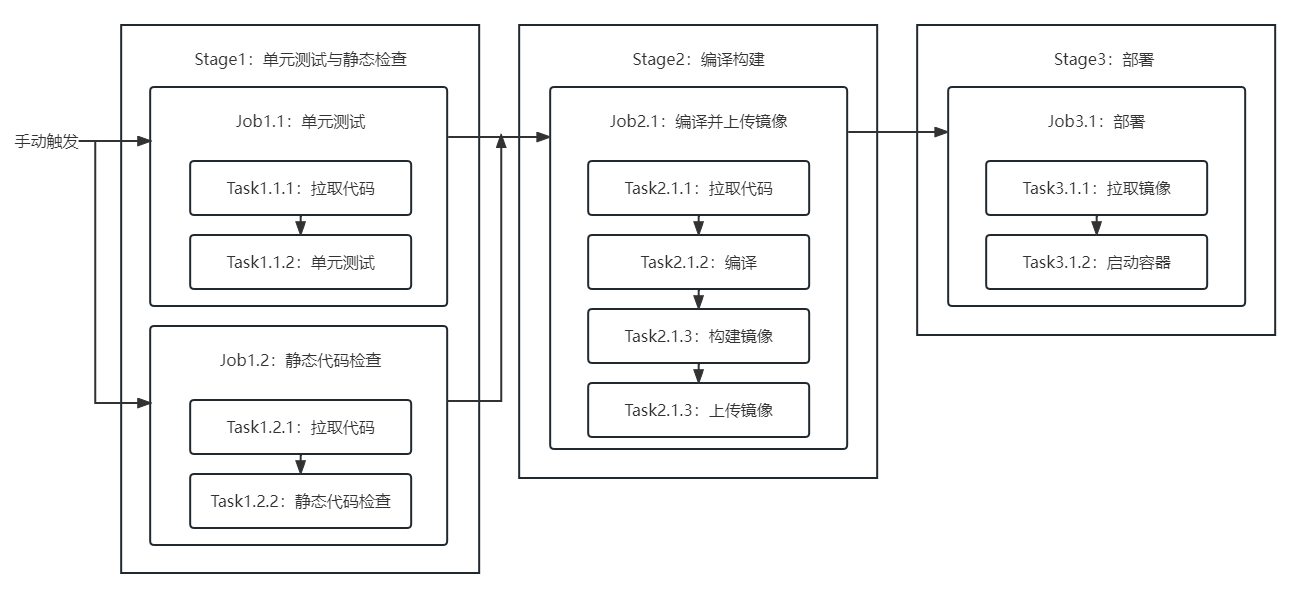
\includegraphics[width=1\textwidth]{流水线示意图.png}
  \caption{流水线示意图}
  \label{fig:流水线示意图}
\end{figure}



\subsection{人为干预需求}
在实际业务的集成与交付中,为满足用户对流水线的复杂操作需求,提高流水线的灵活度,CI/CD调度系统需要支持用户在流水线执行过程中主动对流水线的执行情况进行干预;
干预行为主要包括:

\paragraph{手动触发(Trigger)}
流水线的触发通常分为自动触发和手动触发两种方式

\paragraph{取消(Cancel)}
当用户在流水线的运行过程中,意识到流水线的后续执行会产生自己不期望的后果时,CI/CD调度系统应支持用户将其取消。
注意,当阶段或作业被取消后,系统应视为其已经失败,应阻止与其串行的后续阶段或作业的继续执行。

\paragraph{重试(Retry)}
流水线中某个作业的失败往往不是必现的,当用户认为某个失败的作业并非源于配置或者代码本身,而是因为运行环境、网络稳定性等因素导致失败时,CI/CD调度系统应支持用户将其重试。

\paragraph{跳过(Skip)}
通常来说,一条精心配置的流水线包含非常多的阶段和作业。但复用这条流水线的各个用户的需求可能各不相同。
当某个阶段或者作业用户认为没有必要执行,或者运行时间过长用户不希望再等待时,CI/CD调度系统应支持用户将其跳过。
注意,与“取消”操作相反,当阶段或作业被跳过后,系统应视为其已经成功,应立即继续与其串行的后续阶段或作业的继续执行。

\paragraph{人工审核(Review)}
当流水线运行到某个阶段或某个作业时,为确保后续按期望执行,并保证流水线产物的质量,CI/CD调度系统应支持用户在某个阶段或作业开始前,加入人工审核的环节。
同时,这一功能应支持流水线的编辑者自行设置审核人和审核的通过条件,比如设置了两位部门领导作为审核人,当任意一位审核人进入系统并点击“批准”后,该阶段或作业即开始执行。

以上人工干预行为分别适用于一个或多个流水线中的子概念(流水线、阶段、作业和任务),依据对常见业务场景的分析,各个概念应支持的人工干预行为如表~\ref{tab:各个子概念应支持的人为干预行为表}:
\begin{table}[h]
  \centering
  \caption{各个子概念应支持的人为干预行为表}
  \label{tab:各个子概念应支持的人为干预行为表}
  \begin{tabular}{cl}
    \toprule
    子概念   & 人为干预行为                                     \\
    \midrule
    流水线 & 手动触发、取消 \\
    阶段      & 人工审核、取消、重试、仅重试阶段中失败作业   \\
    作业      & 手动触发、人工审核、取消、跳过、重试      \\
    任务       & 不允许人为干预       \\
    \bottomrule
  \end{tabular}
\end{table}

\subsection{状态流转需求}
在流水线的执行过程中,流水线中的每个子概念都在不同的状态间流转,通常来说应有如下状态:
就绪中(Pending)、执行中(Running)、执行成功(Success)、执行失败(Failed)、被跳过(Skipped)、被取消(Canceled)。
各个状态的具体解释如表~\ref{tab:状态解释表}。
\begin{table}[h]
  \centering
  \caption{状态解释表}
  \label{tab:状态解释表}
  \begin{tabular}{cl}
    \toprule
    状态           & 解释                                     \\
    \midrule
    就绪中         & 一切准备工作就绪,等待被自动执行、手动执行或审核通过\\
    执行中         & 正在被执行                 \\
    执行成功       & 顺利执行完毕后的状态        \\
    执行失败       & 执行过程中出错后的状态       \\
    被跳过         & 被用户人为干预执行“跳过”后的状态         \\
    被取消         & 被用户认为干预执行“取消”后的状态         \\
    \bottomrule
  \end{tabular}
\end{table}
以上状态适用于流水线中的各个子概念。

CI/CD调度系统需要保障流水线作业能够进行正确的状态流转,以保证用户能够正确、及时地得知流水线的执行情况。
同时,状态的正确流转也是流水线能按照正确逻辑链路执行的保证,系统需要结合当前流水线内各个子概念的状态,结合用户的人为操作,来判断流水线接下来的状态。
图~\ref{fig:流水线作业状态图}以作业为例,描述了其状态转移流程。

\begin{figure}[h]
  \centering
  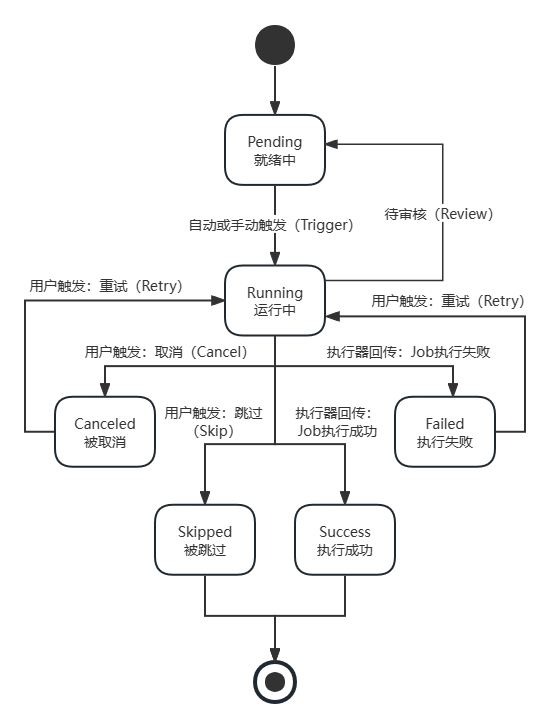
\includegraphics[width=0.8\textwidth]{流水线作业状态图.png}
  \caption{流水线作业状态图}
  \label{fig:流水线作业状态图}
\end{figure}


\subsection{自动触发需求}
自动化是CI/CD流水线提高软件团队研发效能的保证。通常来说,用户会希望某个指定仓库的代码出现变更的时候,CI/CD系统中的流水线便能自动触发。
系统能够某种感知或监听

\subsection{流水线作业合理调度需求}

作业是流水线执行器中执行的最小单位,CI/CD调度器作为流水线配置与作业实际执行环境的中间环节,需要从作业排队、一致性分发、统一调度等方面保证作业的合理调度。

首先,系统需要保证作业的执行顺序与其被调度的顺序一致,即先来先执行。其次,当相当数量的作业被调度,超过了执行器的承载能力时,系统应能保证作业的阻塞等待,当前执行的作业结束执行后,再执行阻塞中的作业。
以上两点需求业内往往借助开源的消息队列服务实现,如Redis、RocketMq等,借助消息队列先进先出和持久化的特性,保证了作业的调度顺序和阻塞等待。

然后,系统需要完成流水线作业的分配任务,将作业能够合理的分配给不同的作业执行模块。
当调度器判断应该调度某个作业时,CI/CD调度器将根据流水线配置时用户预填写的内容封装作业信息,再交付给执行器执行任务。
这一特性往往通过消息队列中消息的Tag来实现对作业的精确分配。
同时,系统需要能够保证一个作业只能被一个执行器所执行,不能被多个执行器重复执行。


\section{非功能性需求}



除功能性需求外,系统需要满足以下非功能需求:

\paragraph{高性能}
本系统致力于提高效能,提升用户的研发效率,需要保证优秀的性能和较短的响应时间。
当用户进行流水线管理时,对流水线的增删改查应在1s内完成;
当用户人为干预流水线时,系统应在2s内给予用户反馈;
当流水线中阶段、作业或者任务的状态发生改变时,应在5s对用户进行展示。

\paragraph{高可用性}
CI/CD流水线系统的可靠性和稳定性尤为重要,一旦直接影响整个企业的开发人员、测试人员和运维人员,阻塞代码合并、业务提测、系统发布等流程。
依据业界常用指标,本系统需要至少达到99.99\%的可用性。
换算成服务时间则根据公式:服务可用率=成功调用数/总调用数,系统每一年的时间内,服务总中断时间不能超过52分钟。

\paragraph{高易用性}
本系统应提供友好的交互逻辑,让缺乏相关知识背景的用户能够快速找到流水线的编辑与配置方式;
同时,由于CI/CD流水线通常有着复杂的层级与结构,系统应提供所见即所得的流水线拓扑结构界面,以便用户查看和调整;
最后,流水线的执行过程中应提供入口,将各个作业的运行日志可视化地展示给用户,方便用户时刻监控流水线作业的执行情况。

\paragraph{高安全性}
流水线中的作业往往会对其对应的系统产生影响,如发布新版本、发送通知等等。
为避免产生不期望的后果,系统应对流水线的触发以及各种操作进行严格的权限控制。

\subsection{二级节标题}

\subsubsection{三级节标题}

\paragraph{四级节标题}

\subparagraph{五级节标题}

本模板 \pkg{ustcthesis} 是中国科学技术大学本科生和研究生学位论文的 \LaTeX{}
模板, 按照《\href{https://gradschool.ustc.edu.cn/static/upload/article/picture/ce3b02e5f0274c90b9331ef50ae1ac26.pdf}
{中国科学技术大学研究生学位论文撰写手册}》(以下简称《撰写手册》)和
《\href{https://www.teach.ustc.edu.cn/?attachment_id=13867}
{中国科学技术大学本科毕业论文(设计)格式}》的要求编写。

Lorem ipsum dolor sit amet, consectetur adipiscing elit, sed do eiusmod tempor
incididunt ut labore et dolore magna aliqua.
Ut enim ad minim veniam, quis nostrud exercitation ullamco laboris nisi ut
aliquip ex ea commodo consequat.
Duis aute irure dolor in reprehenderit in voluptate velit esse cillum dolore eu
fugiat nulla pariatur.
Excepteur sint occaecat cupidatat non proident, sunt in culpa qui officia
deserunt mollit anim id est laborum.



\section{脚注}

Lorem ipsum dolor sit amet, consectetur adipiscing elit, sed do eiusmod tempor
incididunt ut labore et dolore magna aliqua.
\footnote{Ut enim ad minim veniam, quis nostrud exercitation ullamco laboris
  nisi ut aliquip ex ea commodo consequat.
  Duis aute irure dolor in reprehenderit in voluptate velit esse cillum dolore
  eu fugiat nulla pariatur.}
